\documentclass[12pt]{article}

% Users of the {thebibliography} environment or BibTeX should use the
% scicite.sty package, downloadable from *Science* at
% www.sciencemag.org/about/authors/prep/TeX_help/ .
% This package should properly format in-text
% reference calls and reference-list numbers.

%\usepackage{scicite}

% Use times if you have the font installed; otherwise, comment out the
% following line.
\usepackage{url}
\usepackage{times}
\usepackage{graphicx}
\graphicspath{ {./images/} }
\usepackage{mathptmx}
\usepackage[sort]{natbib}
\usepackage{fancyhdr}
\usepackage{bm,amsmath,tikz,bbm,amsfonts,nicefrac,latexsym,amsmath,amsfonts,amsbsy,amscd,amsxtra,amsgen,amsopn,bbm,amsthm,amssymb, enumerate, appendix, listings,subcaption}
\usepackage{pifont}
\usepackage{graphicx}
%\usepackage[margin=0.5in]{geometry}
\usepackage[nottoc,numbib]{tocbibind}
\usepackage[a4paper,left=2cm,right=2cm, bottom=1cm]{geometry}


% The preamble here sets up a lot of new/revised commands and
% environments.  It's annoying, but please do *not* try to strip these
% out into a separate .sty file (which could lead to the loss of some
% information when we convert the file to other formats).  Instead, keep
% them in the preamble of your main LaTeX source file.


% The following parameters seem to provide a reasonable page setup.

\topmargin 0.0cm
\oddsidemargin 0.2cm
\textwidth 16cm 
\textheight 21cm
\footskip 1.0cm


%The next command sets up an environment for the abstract to your paper.

\newenvironment{sciabstract}{%
	\begin{quote} \bf}
	{\end{quote}}


% If your reference list includes text notes as well as references,
% include the following line; otherwise, comment it out.

\renewcommand\refname{References and Notes}

% The following lines set up an environment for the last note in the
% reference list, which commonly includes acknowledgments of funding,
% help, etc.  It's intended for users of BibTeX or the {thebibliography}
% environment.  Users who are hand-coding their references at the end
% using a list environment such as {enumerate} can simply add another
% item at the end, and it will be numbered automatically.

\newcounter{lastnote}
\newenvironment{scilastnote}{%
	\setcounter{lastnote}{\value{enumiv}}%
	\addtocounter{lastnote}{+1}%
	\begin{list}%
		{\arabic{lastnote}.}
		{\setlength{\leftmargin}{.22in}}
		{\setlength{\labelsep}{.5em}}}
	{\end{list}}


% Include your paper's title here

\title{Senior Year Project} 


% Place the author information here.  Please hand-code the contact
% information and notecalls; do *not* use \footnote commands.  Let the
% author contact information appear immediately below the author names
% as shown.  We would also prefer that you don't change the type-size
% settings shown here.

\author
{\\
	Project Supervisor: Dr. Zahra Lakdawala
	\\
	Author: Muhammad Affan
	\\
	\normalsize{$^{1}$Department of Mathematics, Lahore University of Management and Sciences}
	\\
}



% Include the date command, but leave its argument blank.

\date{}



%%%%%%%%%%%%%%%%% END OF PREAMBLE %%%%%%%%%%%%%%%%



\begin{document} 
	
	% Double-space the manuscript.
	
	\baselineskip24pt
	
	% Make the title.
	
	\maketitle 
	
	
	

	\newpage	
	\tableofcontents	
	\newpage
		

		

	
	
	
	% Place your abstract within the special {sciabstract} environment.
	

	
	
	
	% In setting up this template for *Science* papers, we've used both
	% the \section* command and the \paragraph* command for topical
	% divisions.  Which you use will of course depend on the type of paper
	% you're writing.  Review Articles tend to have displayed headings, for
	% which \section* is more appropriate; Research Articles, when they have
	% formal topical divisions at all, tend to signal them with bold text
	% that runs into the paragraph, for which \paragraph* is the right
	% choice.  Either way, use the asterisk (*) modifier, as shown, to
	% suppress numbering.
	
	\section{The Black-Scholes Model}
	
	Black-Scholes is a pricing model used to determine the fair price or theoretical value for a call or a put option based on six variables such as volatility, type of option, underlying stock price, time, strike price, and risk-free rate. The quantum of speculation is more in case of stock market derivatives, and hence proper pricing of options eliminates the opportunity for any arbitrage. There are two important models for option pricing – Binomial Model and Black-Scholes Model. The model is used to determine the price of a European call option, which simply means that the option can only be exercised on the expiration date.
	
	The Black-Scholes model allows us the calculate the price of European call and put options.The value of a call option, $f_c$, and a put option, $f_p$, are given by the following formulae;
	

\begin{align}
f_c &= S\Phi(d_1) - K \mathrm{e}^{-rT}\Phi(d_2)\label{eq:1}, \\
f_p &= K\mathrm{e}^{-rT}\Phi(-d_2) - S \Phi(-d_1).
\end{align}
\begin{align}
	d_1 &= \frac{\log(S/K)+(r+\sigma^2/2)T}{\sigma \sqrt{T}} \label{bsdii1}, \\
	d_2 &= \frac{\log(S/K)+(r-\sigma^2/2)T}{\sigma \sqrt{T}} = d_1 - \sigma. \sqrt{T}.
\end{align}
	
	
	

\begin{itemize}
	\item[] C = Call option price 
	\item[] S = Current stock price
	\item[] K = Strike price of the option
	\item[] r = risk-free interest rate (a number between 0 and 1)
	\item[] $\sigma$ = volatility of the stocks return (a number between 0 and 1)
	\item[] t = time to option maturity (in years)
	\item[] N = normal cumulative distribution function
\end{itemize}


	
	
	\subsection{The Black-Scholes Assumptions}
	
\textbf{Lognormal distribution:} The Black-Scholes-Merton model assumes that stock prices follow a lognormal distribution based on the principle that asset prices cannot take a negative value; they are bounded by zero.

\noindent
\textbf{No dividends:} The BSM model assumes that the stocks do not pay any dividends or returns.

\noindent
\textbf{Expiration date:} The model assumes that the options can only be exercised on its expiration or maturity date. Hence, it does not accurately price American options. It is extensively used in the European options market.

\noindent
\textbf{Random walk:} The stock market is a highly volatile one, and hence, a state of random walk is assumed as the market direction can never truly be predicted.

\noindent
\textbf{Frictionless market:} No transaction costs, including commission and brokerage, is assumed in the BSM model.

\noindent
\textbf{Risk-free interest rate:} The interest rates are assumed to be constant, hence making the underlying asset a risk-free one.

\noindent
\textbf{Normal distribution:} Stock returns are normally distributed. It implies that the volatility of the market is constant over time.

\noindent
\textbf{No arbitrage:} There is no arbitrage. It avoids the opportunity of making a riskless profit.
	





\subsection{Example}
You want to buy an IBM European call option with a strike price of \$210. The stock is currently trading at a price of \$208.99 . You calculate the volatility of the stock to be 17\%. 
The rate at which you can borrow and lend money is 5\% (this is the risk-free interest rate). 
The time to maturity of the option is 77 days. What price should you pay (per share) for the option contract?

$$\mathrm d_1= \frac{1}{0.17 \sqrt{0.21095}} \left[\ln{\left(\frac{208.99}{210}\right)} + 0.21095\left(0.05 + \frac{0.17^2}{2} \right) \right]=0.052$$
$$\mathrm d_2= \frac{1}{0.17 \sqrt{0.21095}} \left[\ln{\left(\frac{208.99}{210}\right)} + 0.21095\left(0.05 - \frac{0.17^2}{2} \right) \right]=-0.027$$

Now that we've calculated $\mathrm d_1$ and $\mathrm d_2$ we will calculate, $f_c$, the value of European call option.




Now we plug these in equation \eqref{eq:1} to calculate the price of the call option.


$$\mathrm f_c= 208.99\Phi(0.052) - 210\mathrm{e}^{0.7*0.21095}\Phi(-0.027) = 7.10$$
 
Then value of call-option after 77 days comes out to be \$7.10. The value is verified using online Black-Scholes calculator.

\includegraphics[width=16cm]{P2}

\subsection{Greeks}
"Greeks" is a term used in the options market to describe the different dimensions of risk involved in taking an options position. These variables are called Greeks because they are typically associated with Greek symbols. Each "Greek" variable is a result of an imperfect assumption or relationship of the option with another underlying variable. Traders use different Greek values, such as delta, theta, and others, to assess options risk and manage option portfolios. 


	
	

\section{Black-Scholes Option Calculator} \label{The Black-Scholes Model}

The main purpose for making Black-Scholes Calculator is to check our analytical solution obtained from Black-Scholes model against the numerical solution obtained after solving Black-Scholes Equation.The implementation of  Black-Scholes Calculator required two things mainly the analytical and numerical solution of the Black-Scholes equation.Analytical solution is straightforward and it can be obtained from the formula given in  \ref{eq:2}. However Obtaining Numerical Solution is not an easy task. A numerical scheme is required which ensures a stable solution for the Black-Scholes equations.

\begin{equation}
	\frac{\partial \mathrm C}{ \partial \mathrm t } + \frac{1}{2}\sigma^{2} \mathrm S^{2} \frac{\partial^{2} \mathrm C}{\partial \mathrm S^2}
	+ \mathrm r \mathrm S \frac{\partial \mathrm C}{\partial \mathrm S}\ =
	\mathrm r \mathrm C 
	\label{eq:5}
\end{equation}

An important thing to consider is the choice of our numerical scheme. Not all Numerical Schemes ensure a stable solution for the Black-Scholes Equation.Some common schemes used to solve BS equations are Implicit Method, Explicit Method and Crank–Nicolson method.
Usually the Crank–Nicolson scheme is the most accurate scheme for small time steps. For larger time steps, the implicit scheme works better since it is less computationally demanding. The explicit scheme is the least accurate and can be unstable, but is also the easiest to implement and the least numerically intensive. Implicit Method was used for making this calculator.

	
\subsection{Finite Difference Method}

%all this from 
\label{fdms}
We may use finite difference methods to solve the Black-Scholes equation and therefore price options. We first recall a few basic results about Taylor series and finite difference methods. Let $f(x)$ be a function that is twice differentiable, we know using Taylors theorem that,
\begin{align}
	&f''(x) = \frac{1}{(\Delta x)^2} (f(x + \Delta x) + f(x - \Delta x) - 2f(x))  + \mathcal{O}((\Delta x)^2)\label{C1},\\
	&f'(x) = \frac{1}{2\Delta x}(f(x + \Delta x) + f(x - \Delta x)) + \mathcal{O}((\Delta x)^2). \label{eq:7}
\end{align}
These are well known approximation to us, for the single variable case. We know that Equation (\ref{eq:7}) is known as the \emph{central difference approximation}, we are also familiar with the \emph{forward difference approximation} and \emph{backward difference approximation}, which respectively are,
\begin{align*}
	f'(x) = \frac{1}{\Delta x}(f(x + \Delta x) -f(x)), \\
	f'(x) = \frac{1}{\Delta x}(f(x) -f(x-\Delta x)).
\end{align*}
\cite{bworld1}
\subsection{Terminal and Boundary Condition}



Say that we truncate the plane so that $S \in [S_{\min}, S_{\max}]$, we still consider $t \in [0,T]$. Then we have the boundary and terminal conditions for a European option, are given in Table \ref{tab:bc'st}, where $V(S,t)$ is the value of the option at stock price $S$ and at time $t$.
\begin{table}[ht]
	\centering
	\begin{tabular}{|l||c|c|c|c|}
		\hline
		Boundary & European Call & European Put  \\ \hline
		$t = T$ & $V(S,T) = \max(S_{\min} + j\Delta S - K,0)$ & $V(S,T) = \max(K-S_{\min} - j\Delta S,0)$  \\
		$S=S_{\min}$ & $V(S_{\min},t) = \max(S_{\min}-K,0)$ & $V(S_{\min},t) = K\mathrm{e}^{-r(T-t)}$   \\
		$S=S_{\max}$ & $V(S_{\max},t) = \max(S_{\max} - K,0)$ & $V(S_{\max},t) = \max(K-S_{\max},0)$  \\\hline
	\end{tabular}
	\caption{\label{tab:bc'st} The conditions at each boundary of the gird for a European option }
\end{table}
These boundary and side conditions are found by using the payoff function at the necessary points. The points of interest are at the termination date and the sides as this is where we have truncated our plane to, hence we arrive at the above. 
\cite{bworld1}
\subsection{Implicit-Method}

When approximating the Black-Scholes differential equation we use a backwards difference approximation for the $\frac{\partial f}{\partial S}$ derivative, a forward difference approximation for the  $\frac{\partial f}{\partial t}$ and a central difference approximation for the $\frac{\partial^2 f}{\partial S^2}$ derivative. Hence, the Black-Scholes equation becomes, 

\begin{align}
	\frac{f_{i+1,j} - f_{i,j}}{\Delta t} + r j \Delta S\frac{f_{i,j+1} - f_{i,j-1}}{2\Delta S} + \frac{1}{2} \sigma^2 (j\Delta S)^2\frac{f_{i,j+1} + f_{i,j-1} - 2 f_{i,j}}{\Delta S^2} = rf_{i,j}. \label{IM1}
\end{align}

We may then rearrange this to find coefficients for the $f_{i,j-1}$, $f_{i,j}$ and $f_{i, j+1}$. This yields that (\ref{IM1}) is now,
\begin{align}
	a_jf_{i,j-1} + b_jf_{i,j} + c_jf_{i,j+1} = f_{i+1,j} \label{FDMI}
\end{align}
where,
\begin{align*}
	a_j &= \frac{1}{2}(r-q)j\Delta t - \frac{1}{2}\sigma^2j^2\Delta t, \\
	b_j &= 1 + \sigma^2 j^2 \Delta t + r \Delta t, \\
	c_j &= -\frac{1}{2}(r-q)j\Delta t - \frac{1}{2}\sigma^2j^2\Delta t.
\end{align*}
Note that these constants are independent of $S$. This is because the $\Delta S$ and $\Delta S^2$ introduced by the derivatives are the same $\Delta S$ that we are considering the option over in any given triangle. Thus once we discretize the plane we have cancellation resulting in the above relationships.

Now we need to solve this so that we can calculate the value of our option at $t=0$ i.e. $i=0$. For a European option we begin by considering $i = N-1$ in (\ref{FDMI}), for $j = 1,\dots,M-1$. Thus we have $M-1$ simultaneous equations to solve. If we write out a few of these,
\begin{align*}
	a_1 f_{N-1,0} + b_1 f_{N-1,1} + c_1f_{N-1,2} &= f_{N,1} \\
	a_2 f_{N-1,1} + b_2 f_{N-1,2} + c_2f_{N-1,3} &= f_{N,2} \\
	&\vdots \\
	a_{M-2}f_{N-1,M-3} + b_{M-2}f_{N-1,M-2} + c_{M-2}f{N-1,M-1} &= f_{N,M-1}\\
	a_{M-1}f_{N-1,M-2} + b_{M-1}f_{N-1,M-1} + c_{M-1}f{N-1,M} &= f_{N,M}.
\end{align*}

Note that all the $f_{i,N}$ are known from the boundary conditions. Furthermore the terms $a_1f_{N-1,0}$ and $c_{M-1}f_{N-1,M}$ are known from the boundary conditions. We may then express our system with unknowns on the left and knowns on the right.

\begin{align*}
	\begin{pmatrix}
		b_{1} & c_{1} &&&&  \\
		a_{2} & b_{2} & c_2 &&&\\
		& a_{3} & b_{3} & c_3 &&\\
		&& \ddots & \ddots  & \ddots&\\
		&&& a_{M-2}&b_{M-2}&c_{M-2} \\
		&&&&a_{M-1}&b_{M-1} 
	\end{pmatrix}
	\begin{pmatrix}
		f_{N-1,1} \\
		f_{N-1,2} \\
		f_{N-1,3} \\
		\vdots \\
		f_{N-1,M-2}  \\
		f_{N-1,M-1}
	\end{pmatrix}
	= 
	\begin{pmatrix}
		f_{N,1} \\
		f_{N,2} \\
		f_{N,3} \\
		\vdots \\
		f_{N,M-2}  \\
		f_{N,M-1}
	\end{pmatrix}
	+ 
	\begin{pmatrix}
		-a_1f_{N-1,0} \\
		0 \\
		0 \\
		\vdots \\
		0  \\
		-c_{M-1}f_{N-1,M}
	\end{pmatrix}.
\end{align*}
Allowing $A$ to be the leftmost matrix and $F_i$ to be the leftmost vector so that $F_{i+1}$ is the second leftmost vector and $B_i$ to be the rightmost vector we have that,
\begin{align}
	AF_i = F_{i+1} + B_i. \label{MF}
\end{align}
In the matrix form above we have taken $i=N-1$ however we note that this is true for arbitrary $i$.
We may solve these using the tridiagonal matrix algorithm for $N-1$, then the $F_{N-1}$ we have found is used in (\ref{MF}) with $i=N-2$ to find $F_{N-2}$. We may continue doing this until we reach $i=0$ and we may find the value of our option at this point.
\cite{bworld1}

\subsection{Results}
 After solving the Black-Scholes equation by analytical and numerical schemes we obtain the following results which tells us that both are approximately the same. One can always change other parameters like volatility, risk-free rate, Time of maturity e.t.c to observe the changes in the solution curve.
 
 
 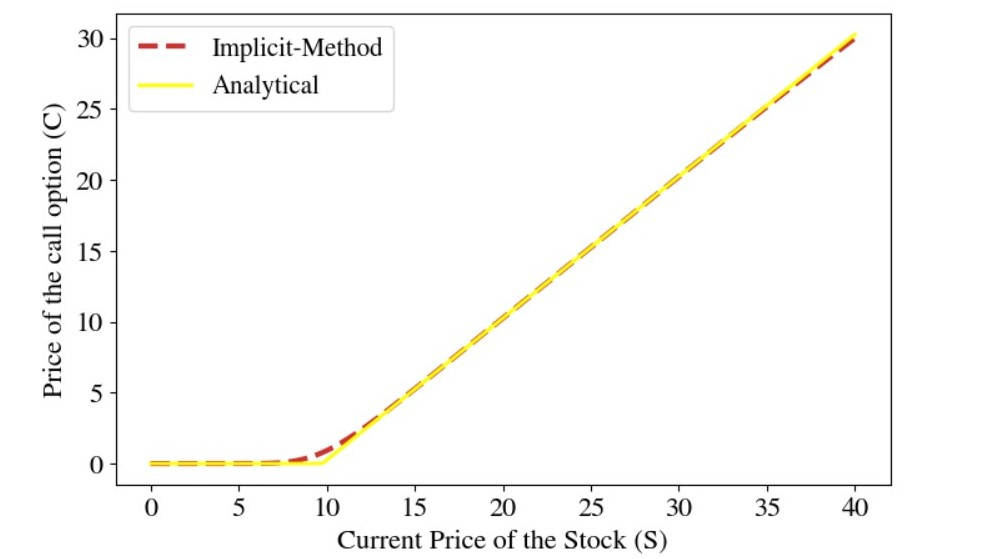
\includegraphics[width=14cm]{P1}
 \subsection{Benchmarks}
 
 The results were quite close if we look at the graph in the result section. But we need to see results over a long period at different time steps to see how our numerical and analytical method perform. 
 The picture below shows the options price at different time-steps obtained using the implicit method.
 
  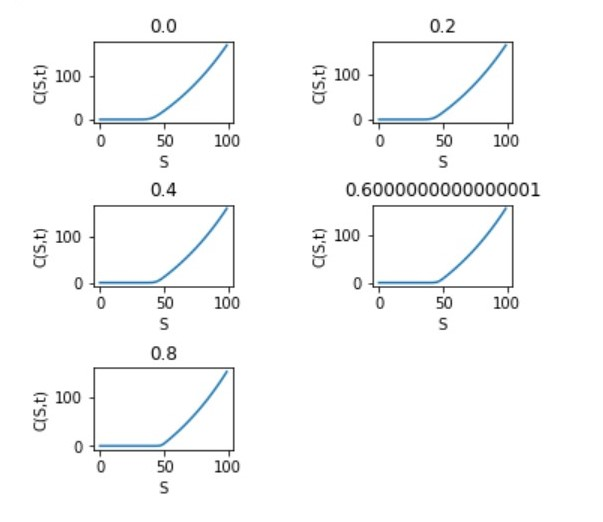
\includegraphics[width=10cm]{p3}
  
The same parameters were used for analytical method and the following results were obtained. 

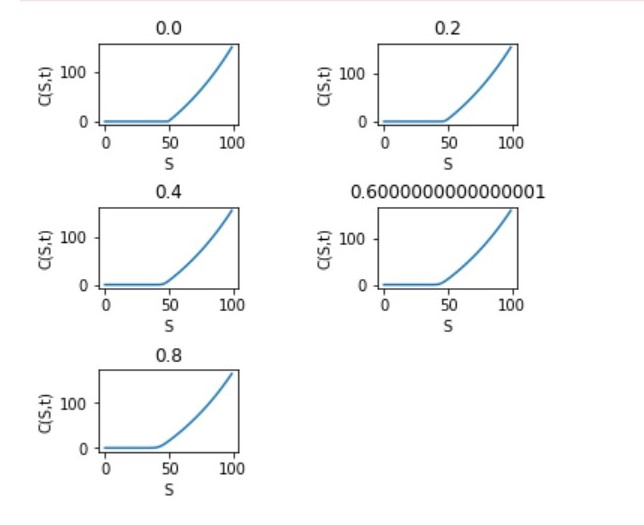
\includegraphics[width=10cm]{p4}

 The results are quite close but the parameters used were hypothetical. So in order to get a better sense of the results introducing some non-linearity in the parameters like volatility will help us identify the stability of these methods.
 
  \subsection{Limitations of the Black-Scholes Model}
  There are limitations on the Black-Scholes model, which is one of the most popular models for options pricing. Some of the standard limitations of the Black-Scholes model are:
 \begin{itemize}
  \item Assumes constant values for the risk-free rate of return and volatility over the option duration. None of those will necessarily remain constant in the real world.
  
  \item Assumes continuous and costless trading—ignoring the impact of liquidity risk and brokerage charges.
  
  \item Assumes stock prices to follow a lognormal pattern, e.g., a random walk (or geometric Brownian motion pattern), thus ignoring large price swings that are observed more frequently in the real world.
  
  \item Assumes no dividend payout—ignoring its impact on the change in valuations.
  
  \item Assumes no early exercise (e.g., fits only European options). That makes the model unsuitable for American options.
  \cite{seth_2022}
  \end{itemize}
  
\section{Introducing non-linearity in volatility}

 \subsection{Implied Volatility}
 Volatility is a major factor in the price of an option. When thinking of volatility it is useful to think of it as the range of potential future stock prices.Implied volatility is an estimate of the future variability for the asset underlying the options contract. The Black-Scholes model is used to price options. The model assumes the price of the underlying asset follows a geometric Brownian motion with constant drift and volatility.
 
 As with any equation, Black-Scholes can be used to determine any single variable when all the other variables are known.To calculate implied volatility i took options data of NFLX(Netflix) to get a varying volatility. We can look at calculating implied-volatility as a minimization problem. Below we minimize the absolute difference between the market price and the Black-Scholes price.We have bounded this minimization such that the volatility is less than 600 \%.
 
 
\begin{align}
	implied volatility=argmin_{\sigma \in(0,6]} |Vmarket  - VBS(S,K,T,r,\sigma)|
\end{align}

Now lets calculate the implied volatility for NFLX. The below mentioned image shows the implied-volatility from the real data and implied-volatility calculated using Newton-Raphson method. \cite{bworld}

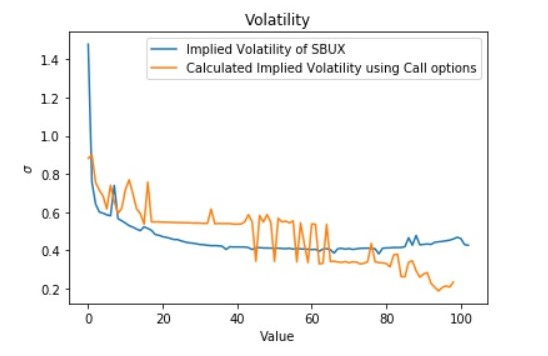
\includegraphics[width=12cm]{p6}

There is a significant difference at the start but the calculated Implied Volatility follows the general trend of original volatility. Our Target was to get a non-linear profile of the volatility and we have now got one. Lets see how to option price look like with this volatility. 

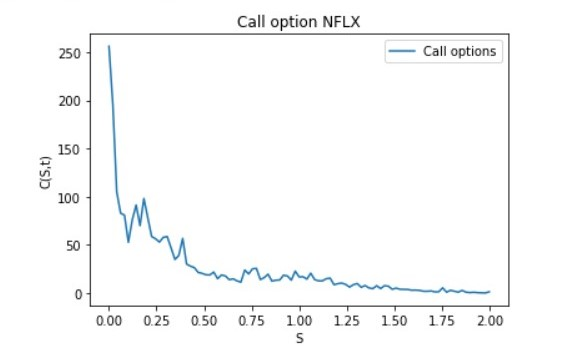
\includegraphics[width=12cm]{p7}

We can see that our call-option is decaying over the time but there is non-linearity is the decaying of the option. So we have obtained non-linear profiles for our Black-Scholes model.



\bibliographystyle{plain}
\bibliography{Bib}	


	
	
\end{document}